\documentclass{beamer}

% -----------------------------------------------------------------------------
% Packages
% -----------------------------------------------------------------------------

\usepackage{graphicx}   % For including images (e.g., QR codes)
\usepackage{hyperref}   % For clickable hyperlinks
\usepackage{xcolor}     % For defining custom colors
\usepackage{iexec}     % Uncomment if you want to use Git commit hash for document version
\usepackage{tcolorbox}  % For creating colored boxes for organization and emphasis
\usepackage{qrcode}     % For generating QR codes directly in LaTeX
\usepackage{pifont}     % For using dingbat symbols (e.g., checkmarks for compatibility)

\newcommand{\gitAbbrevHash}{\iexec{git rev-parse --short HEAD}} % Command to get Git commit hash for versioning (requires iexec)

% -----------------------------------------------------------------------------
% Hyperlink Colors Configuration
% -----------------------------------------------------------------------------
% Sets colors for hyperlinks to improve readability
\hypersetup{
    colorlinks=true,   % Enables colored links instead of default boxed links
    linkcolor=blue,    % Color for internal document links (e.g., TOC)
    urlcolor=cyan      % Color for external links (e.g., URLs)
}

% -----------------------------------------------------------------------------
% Footer Configuration
% -----------------------------------------------------------------------------
% Customizes the footer to display organization, workshop name, semester, and page number
\setbeamertemplate{footline}{%
  \leavevmode%
  \hbox{
    % Left: Organization Name
    \begin{beamercolorbox}[wd=.35\paperwidth,ht=2.25ex,dp=1ex,leftskip=.3cm]{author in head/foot}%
      Wireless Club at Northeastern University%
    \end{beamercolorbox}%
    % Center: Workshop Name
    \begin{beamercolorbox}[wd=.20\paperwidth,ht=2.25ex,dp=1ex,center]{author in head/foot}%
      Adv. Embedded Workshop%
    \end{beamercolorbox}%
    % Center: Semester Information
    \begin{beamercolorbox}[wd=.15\paperwidth,ht=2.25ex,dp=1ex,center]{author in head/foot}%
      Fall 2024%
    \end{beamercolorbox}%
    % Right: Version (Git commit hash) and Page Number
    \begin{beamercolorbox}[wd=.30\paperwidth,ht=2.25ex,dp=1ex,rightskip=.3cm plus1fil]{author in head/foot}%
      Version: \gitAbbrevHash{} \hspace{1em} \insertframenumber/\inserttotalframenumber%
    \end{beamercolorbox}}%
  \vskip0pt%
}

% -----------------------------------------------------------------------------
% Slide: Title Page
% -----------------------------------------------------------------------------
\title{Advanced Embedded Development Workshop}
% \subtitle{Hosted by the Northeastern University Institute of Electrical and Electronics Engineers (IEEE) Club}
\author{Northeastern University Wireless Club - W1KBN}
\date{November 4, 2024}

\begin{document}

% -----------------------------------------------------------------------------
% Slide: Title with QR Code for Sign-In
% -----------------------------------------------------------------------------
\begin{frame}
    \titlepage % Generates the title, subtitle, author, and date
    \vspace{-1cm} % Adjusts spacing to accommodate the QR code
    \begin{center}
        \textbf{Sign in Here:} \\ % Prompt for participants to sign in
        % \includegraphics[width=0.30\textwidth]{images/nuwc-signin-qrcode.png} % Image-based QR code (if needed)
        \qrcode{https://l.w1kbn.org/signin} % Generates QR code for sign-in URL
        \\
        {\small \url{https://l.w1kbn.org/signin}} % Sign-in URL for participants to manually access
    \end{center}
\end{frame}

% -----------------------------------------------------------------------------
% Slide: General Information and Sign-In
% -----------------------------------------------------------------------------
\begin{frame}
    \begin{tcolorbox}[colframe=blue!75!black, colback=blue!10, title=About, center title]
        \begin{itemize}
            \item Regular Meetings: Thursdays, 7 PM @ Hayden Hall, Room 503
            \item Workshops: Mondays, 7 PM @ East Village, Room 010
        \end{itemize}        
    \end{tcolorbox}
    
    \begin{tcolorbox}[colframe=blue!75!black, colback=blue!10, title=QR Codes \& Links, center title]
        \begin{minipage}{0.32\textwidth}
            \centering
            \textbf{Sign in} \\
            \qrcode{https://l.w1kbn.org/signin} \\
            \tiny \url{https://l.w1kbn.org/signin}  % Smaller font for URL
        \end{minipage}
        \begin{minipage}{0.32\textwidth}
            \centering
            \textbf{Slack} \\
            \qrcode{https://neuwireless.slack.com/join/signup} \\
            \tiny \url{https://neuwireless.slack.com/join/signup}
        \end{minipage}
        \begin{minipage}{0.32\textwidth}
            \centering
            \textbf{Mailing List} \\
            \qrcode{http://eepurl.com/gduCIr} \\
            \tiny \url{http://eepurl.com/gduCIr}
        \end{minipage}
        \begin{itemize}
            \item Website: \url{https://nuwireless.org/}
        \end{itemize}
    \end{tcolorbox}
\end{frame}

% -----------------------------------------------------------------------------
% Slide: Workshop Goals
% -----------------------------------------------------------------------------
\begin{frame}
    \frametitle{Workshop Goals}
    \begin{itemize}
        \item Explore the fundamentals of bare-metal programming on the STM32 platform
        \item Gain experience with assembly language for low-level control
        \item Learn to interact with sensors and input devices at a hardware level
        \item Understand the role of the Hardware Abstraction Layer (HAL) for embedded C development
        \item Build a foundation for industry-relevant embedded development techniques
    \end{itemize}
\end{frame}

% -----------------------------------------------------------------------------
% Slide: Workshop Overview
% -----------------------------------------------------------------------------
\begin{frame}
    \frametitle{Workshop Overview}
    \begin{columns}
        \begin{column}{0.55\textwidth}
            \begin{itemize}
                \item Introduction to STM32 and bare-metal programming
                \item Hands-on practice with assembly to control hardware
                \item Setting up and using the embedded C HAL for streamlined development
                \item Working with sensors and input devices directly through registers
                \item Transitioning from low-level assembly to higher-level embedded C workflows
            \end{itemize}
        \end{column}
        \begin{column}{0.4\textwidth}
            \begin{center}
                \includegraphics[width=\textwidth]{images/nuwc-advanced-embedded-workshop-overview.jpg}
            \end{center}
        \end{column}
    \end{columns}
\end{frame}

% -----------------------------------------------------------------------------
% Slide: Bill of Materials (BOM)
% -----------------------------------------------------------------------------
\begin{frame}
    \frametitle{Bill of Materials (BOM)}
    \textbf{A full kit contains:}
    \begin{itemize}
        \item \textbf{Solderless Breadboard}
        \begin{itemize}
            \item Column separation: 0.3 inches
            \item Pin spacing: 0.1 inches
            \item Compatible with 29-20 AWG wire sizes
        \end{itemize}
        \item \textbf{NUCLEO-F031K6 Development Board}
        \item \textbf{LSM6DSOX IMU}
        \item \textbf{USB Cable} (USB-C to USB Micro-B or USB-A to USB Micro-B)
        \item \textbf{STEMMA QT / Qwiic JST SH 4-pin to Premium Male Headers Cable} (4-wire cable)
        \item \textbf{Jumper Wires} (7 pieces)
        \item \textbf{220 $\Omega$ Resistors} (4 pieces, through-hole)
        \item \textbf{LEDs} (4 pieces, any consistent color)
    \end{itemize}
\end{frame}

% -----------------------------------------------------------------------------
% Slide: Software Requirements (1)
% -----------------------------------------------------------------------------
\begin{frame}
    \frametitle{Software Requirements (1)}
    \footnotesize % Set font size to footnotesize for more compact text
    \begin{table}[]
        \begin{tabular}{|p{2cm}|p{3cm}|p{1cm}|p{3.5cm}|} % Define column widths
            \hline
            \textbf{Component} & \textbf{Description} & \textbf{Version} & \textbf{Download Link} \\ \hline
            \textbf{VS Code \newline \ding{192} \ding{193} \ding{194}} & IDE / Text Editor & Latest & \url{https://code.visualstudio.com/} \\ \hline
            \textbf{VS Code Extension: \texttt{Cortex-Debug} \ding{192} \ding{193} \ding{194}} & ARM Cortex-M GDB Debugger support for VS Code & 1.12.1 & \url{https://marketplace.visualstudio.com/items?itemName=marus25.cortex-debug} \\ \hline
            \textbf{GNU Arm Embedded Toolchain \newline \ding{192} \ding{193} \ding{194}} & Compiler/toolchain: \texttt{gcc-arm-none-eabi} & 10.3-2021.10 & \url{https://developer.arm.com/downloads/-/gnu-rm} \\ \hline
            \textbf{CMake \newline \ding{192} \ding{193} \ding{194}} & Build system & Latest & \url{https://cmake.org/download/} \\ \hline
			\textbf{GNU Make \newline \ding{193}} & Build system, should be already installed on Linux/MacOS & Latest & \url{https://gnuwin32.sourceforge.net/packages/make.htm} \\ \hline
        \end{tabular}
    \end{table}
\end{frame}

% -----------------------------------------------------------------------------
% Slide: Software Requirements (2)
% -----------------------------------------------------------------------------
\begin{frame}
    \frametitle{Software Requirements (2)} % Continuation slide title
    \footnotesize % Set font size to footnotesize for more compact text
    \vspace{-2cm} % Reduce vertical space to position content immediately below the title
    \begin{table}[]
        \begin{tabular}{|p{2cm}|p{3cm}|p{1cm}|p{3.5cm}|} % Define column widths
            \hline
            \textbf{Component} & \textbf{Description} & \textbf{Version} & \textbf{Download Link} \\ \hline
            \textbf{J-Link \newline \ding{192} \ding{193}} & Flashing and debugging software & V8.10e & \url{https://www.segger.com/downloads/jlink/} \\ \hline
            \textbf{ST-Link \newline \ding{194}} & Open source toolset for STM32 devices & Latest & Arch/Fedora: \texttt{stlink} or Debian: \texttt{stlink-tools} \\ \hline
            \textbf{Source Code \newline \ding{192} \ding{193} \ding{194}} & Workshop code repo & Latest & \url{https://github.com/jlefkoff/advanced-embedded} \\ \hline
            \textbf{Xcode \newline \ding{192}} & macOS IDE needed for \texttt{make} & Latest & run \newline \tiny\texttt{sudo xcode-select --install} \\ \hline
        \end{tabular}
    \end{table}
        % Compatibility legend for icons/dings used above:
    \textbf{Compatibility Legend:} \ding{192} macOS \hspace{1em} \ding{193} Windows \hspace{1em} \ding{194} Linux
\end{frame}

% -----------------------------------------------------------------------------
% Slide: Wiring Diagram
% -----------------------------------------------------------------------------
\begin{frame}
	\frametitle{Wiring Diagram}
	\begin{center}
		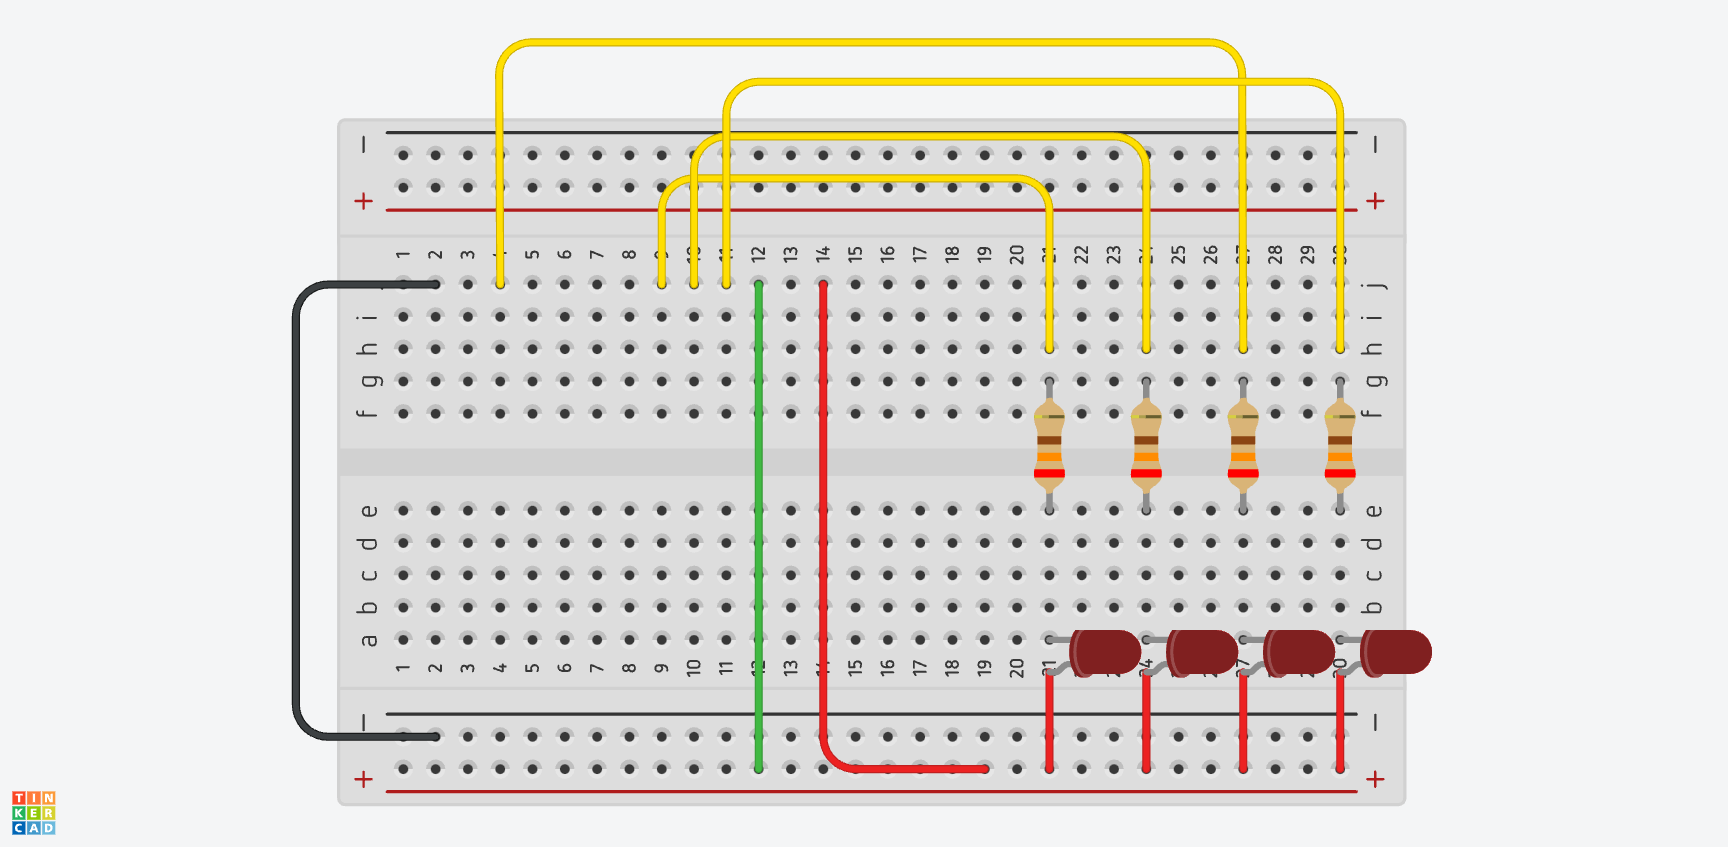
\includegraphics[width=\textwidth]{images/breadboard.png}
	\end{center}
\end{frame}

% -----------------------------------------------------------------------------
% Slide: Theory (1)
% -----------------------------------------------------------------------------
\begin{frame}
    \frametitle{CPU Theory}
    \begin{columns}
        \begin{column}{0.55\textwidth}
			\textbf{Instruction}
			\begin{itemize}
				\item Computer programs consist of many many instructions
				\item Opcode + parameters
			\end{itemize}

			\textbf{Opcodes}
			\begin{itemize}
				\item Each possible CPU operation is assigned a number
				\item Varies between processor families
				\item Difficult to work with
			\end{itemize}
        \end{column}
        \begin{column}{0.4\textwidth}
			\begin{figure*}
				\centering
                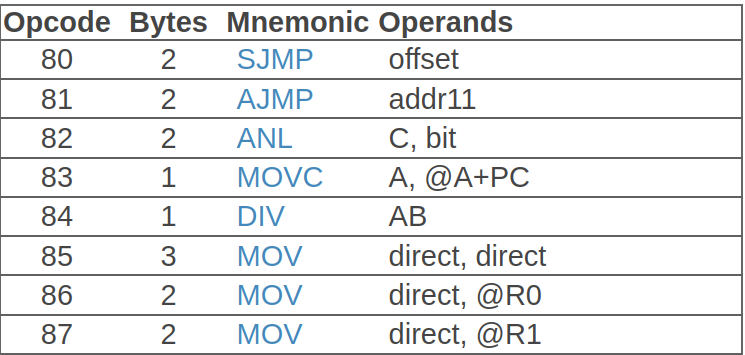
\includegraphics[width=\textwidth]{images/8051_opcodes.png}
				\caption{\small Some Intel 8051 Opcodes}
			\end{figure*}
        \end{column}
    \end{columns}
\end{frame}

% -----------------------------------------------------------------------------
% Slide: Theory (2)
% -----------------------------------------------------------------------------
\begin{frame}
    \frametitle{Assembly Language}
    \begin{columns}
        \begin{column}{0.55\textwidth}
			\textbf{Why Assembly?}
			\begin{itemize}
				\item Human readable opcodes
				\item 1 line of assembly = 1 CPU instruction
			\end{itemize}

			\textbf{Writing Assembly}
			\begin{itemize}
				\item Directives
				\item Labels
				\item Instructions
				\item Comments
			\end{itemize}
        \end{column}
        \begin{column}{0.4\textwidth}
			\begin{figure*}
				\centering
				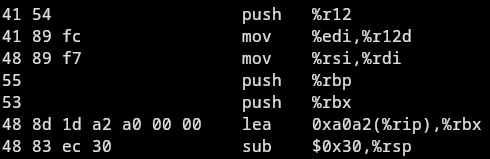
\includegraphics[width=\textwidth]{images/x86_binary.png}
				\caption{\small x86\_64 Assembly Decompilation}
			\end{figure*}

			\vspace{0.5cm}

			\begin{figure*}
				\centering
				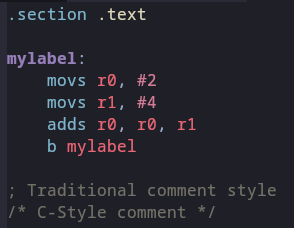
\includegraphics[width=\textwidth]{images/assembly.png}
				\caption{\small ARM Assembly}
			\end{figure*}
        \end{column}
    \end{columns}
\end{frame}

% -----------------------------------------------------------------------------
% Slide: Theory (3)
% -----------------------------------------------------------------------------
\begin{frame}
	\frametitle{Registers vs Stack}
	\textbf{Registers}
	\begin{itemize}
		\item Registers are very fast, but there are not many
		\item Computations are done in registers
		\begin{itemize}
			\item \texttt{movs r0, \#80 // write 80 to r0}
			\item \texttt{movs r1, \#40 // write 40 to r1}
			\item \texttt{adds r0, r0, r1 // r0 = r0 + r1}
		\end{itemize}
		\item \texttt{adds, subs, ands, orrs, eors}
	\end{itemize}

	\textbf{Stack}
	\begin{itemize}
		\item Large in size, but cannot be manipulated directly
		\item Useful for storing values
		\begin{itemize}
			\item \texttt{push \{r0\} // put the value of r0 on the stack}
			\item We can now modify the value of r0 here without losing it
			\item \texttt{pop \{r0\} // get our value back into r0}
		\end{itemize}
		\item First In, First Out!
	\end{itemize}
\end{frame}

% -----------------------------------------------------------------------------
% Slide: Challenge (1)
% -----------------------------------------------------------------------------
\begin{frame}
	\frametitle{Challenge 1}
	\textbf{LED Binary Clock}
	\begin{itemize}
		\item Our program is supposed to show a 4-bit binary clock
		\item However, our LEDs are placed in \textbf{Active Low} configuration
		\begin{itemize}
			\item When we write a 1, the LED turns off
			\item When we write a 0, the LED turns on
		\end{itemize}
		\item Find challenge 1 in \texttt{led.s} and add assembly code to flip the value of \texttt{r0}.
		\item Hint: think logic gates
	\end{itemize}
\end{frame}


% -----------------------------------------------------------------------------
% Slide: Theory (4)
% -----------------------------------------------------------------------------
\begin{frame}
	\frametitle{Subroutines \& Special Registers}
	\textbf{Subroutines}
    \begin{itemize}
        \item Similar to functions
		\begin{itemize}
			\item \texttt{bl mysubroutine}
			\item Writes the return location into register \texttt{lr}
		\end{itemize}
		\item After a subroutine is done, it \textbf{returns} back to where it was called by calling \texttt{bx lr}
		\item What happens if we \texttt{bl} inside a subroutine?
    \end{itemize}
    \textbf{Program Counter}
    \begin{columns}
        \begin{column}{0.55\textwidth}
			\begin{itemize}
				\item Tracks which part of the program we are in
				\item Instead of \texttt{bx lr}, we can load a value to this register
				\item Store old \texttt{lr} on the stack and pop into \texttt{pc} later
			\end{itemize}
        \end{column}
        \begin{column}{0.4\textwidth}
			\begin{figure*}
				\centering
				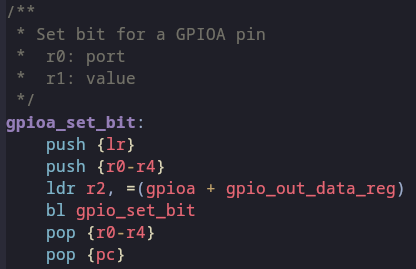
\includegraphics[width=\textwidth]{images/nested_subroutine.png}
				\caption{\small Nested Subroutines}
			\end{figure*}
        \end{column}
    \end{columns}
\end{frame}

% -----------------------------------------------------------------------------
% Slide: Theory (5)
% -----------------------------------------------------------------------------
\begin{frame}
	\frametitle{Memory Locations}
	\textbf{Accessing Memory Locations}
    \begin{itemize}
		\item Like the stack, we cannot manipulate memory values directly
		\item Load into register, modify, then put back
		\begin{itemize}
			\item \texttt{ldr r0, [r1]}
			\item \texttt{str r0, [r1]}
		\end{itemize}
		\item Braces treat value as an memory address
    \end{itemize}
	\textbf{Peripherals}
	\begin{itemize}
		\item Peripherals such as GPIO ports are located in memory
		\item The datasheet has a map of all peripherals
	\end{itemize}
\end{frame}

% -----------------------------------------------------------------------------
% Slide: Challenge (2)
% -----------------------------------------------------------------------------
\begin{frame}
	\frametitle{Challenge 2}
	\textbf{Reading GPIO}
	\begin{itemize}
		\item Find challenge 2 in \texttt{gpio.s} and implement \texttt{gpio\_get\_bit}
		\item Hint: look at our subroutines for inspiration
		\item Hint: \texttt{r1} already has the memory location
	\end{itemize}
\end{frame}

% -----------------------------------------------------------------------------
% Slide: Theory (6)
% -----------------------------------------------------------------------------
\begin{frame}
    \frametitle{Conditional Execution}
	\textbf{Labels}
    \begin{itemize}
        \item Labels can be placed anywhere in code
		\item Most used for subroutines
		\item But also for loops and conditions
    \end{itemize}
    \textbf{If/Else Statements}
    \begin{itemize}
		\item The \texttt{b mylabel} instruction jumps the program to \texttt{mylabel}
		\item The \texttt{beq mylabel} will only jump if the "Zero" flag is set
		\item Performing certain instructions will set flags
		\begin{itemize}
			\item For example: \texttt{cmp r0, \#12}
		\end{itemize}
		\item Some suffixes that can be added to \texttt{b}
		\begin{itemize}
			\item \texttt{\texttildelow eq}: If values are equal
			\item \texttt{\texttildelow le}: If values are not equal
			\item \texttt{\texttildelow lt}: If the first value is less than the second value
			\item \texttt{\texttildelow gt}: If the first value is greater than the second value
			\item See Section 3.3.6 of the Programming Manual for more!
		\end{itemize}
    \end{itemize}
\end{frame}

% -----------------------------------------------------------------------------
% Slide: Challenge (3)
% -----------------------------------------------------------------------------
\begin{frame}
	\frametitle{Challenge 3}
	\textbf{Making the Clock Bidirectional}
	\begin{itemize}
		\item Find challenge 3 in \texttt{vtable.s}
		\item Use the value of GPIOA port 0 to determine which way to count
	\end{itemize}
\end{frame}

% -----------------------------------------------------------------------------
% Slide: Theory (7)
% -----------------------------------------------------------------------------
\begin{frame}
    \frametitle{Other Important Concepts}
	\textbf{Infinite Loop in Main}
    \begin{itemize}
		\item Hardware does not stop executing code
		\item Without a loop, the program will run off into subroutines or uninitialized memory
		\item You must place an infinite loop somewhere in your logic (see \texttt{main.s})
    \end{itemize}
	\textbf{Interrupt Service Routines}
    \begin{columns}
        \begin{column}{0.55\textwidth}
			\begin{itemize}
				\item Interrupt allows the CPU to react to events
				\item ISR labels are placed into a vector table (vtable) at \textbf{specific addresses}
				\item We modified \texttt{isr\_timer} in challenge 3
			\end{itemize}
        \end{column}
        \begin{column}{0.4\textwidth}
			\begin{figure*}
				\centering
				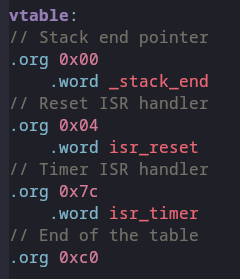
\includegraphics[width=0.7\textwidth]{images/vtable.png}
			\end{figure*}
        \end{column}
    \end{columns}
\end{frame}

% -----------------------------------------------------------------------------
% Slide: Industry Use HAL %
% -----------------------------------------------------------------------------
\begin{frame}
    \frametitle{Industry Use - Hardware Abstraction Layer (HAL)}
    \begin{itemize}
      \item The HAL is a layer of software that abstracts the hardware of a microcontroller.
      \item your time as a dev is more valuable than writing individual register/timer/DMA/SPI/UART code.
      \item HAL provides a higher level of abstraction that allows you to write code that is more portable across different microcontrollers.
    \end{itemize}
\end{frame}


% -----------------------------------------------------------------------------
% Slide: Peripheral Overview
% -----------------------------------------------------------------------------
\begin{frame}
    \frametitle{Inertial Measurement Unit (IMU)}
    \begin{itemize}
      \item The LSM6DSOX is a 6-axis IMU that measures acceleration and angular velocity.
      \item We interface with the IMU using the I2C protocol (talked about it last week).
      \item It has a \dots library! Written by ST. Easy peasy!
    \end{itemize}
\end{frame}


% -----------------------------------------------------------------------------
% Slide: Contact Information
% -----------------------------------------------------------------------------
\begin{frame}
    \frametitle{Contact Us}
    \begin{itemize}
        \item Questions? Feel free to reach out!
        \item Workshop Team Emails: \\
        \{\href{mailto:elarbi.m@northeastern.edu}{elarbi.m}, 
        \href{mailto:aviedov.v@northeastern.edu}{aviedov.v}, 
        \href{mailto:heaney.ma@northeastern.edu}{heaney.ma}\}[at]northeastern[d0t]edu
        \item General Workshop Email: \href{mailto:workshops@nuwireless.org}{workshops}[at]nuwireless[d0t]org
        \item Website: \url{https://nuwireless.org/}
        \item Location: Hayden Hall, Room 503
    \end{itemize}
    \vspace{1cm}
    \begin{flushright}
        \footnotesize{© 2024 Northeastern Wireless Club} \\
        \footnotesize{Design: \href{https://melarbi.com}{Muhammad Elarbi}, based on \LaTeX\ Beamer}
    \end{flushright}
\end{frame}

% -----------------------------------------------------------------------------
% End of Document
% -----------------------------------------------------------------------------
\end{document}
